Dieser Versuch beschäftigt sich mit der Massenspektrometrie. Die Massenspektrometrie beschäftigt sich mit der Trennung gasförmiger Substanzen nach den Massen ihrer Bestandteile. Dazu werden die Bestandteile ionisiert. Die Massenspektrometrie besitzt vielfältige Anwendungen z. B. in der Chemie zur quantitativen und qualitativen Analyse von Substanzen, oder auch in der Industrie.
In diesem Versuch werden unter anderem die Auftrittsenergie von Argon und die Dissoziationsenergien von Stickstoff bestimmt, sowie eine quantitative und qualitative Analyse durchgeführt.

\section{Pumpsysteme}

In diesem Versuch werden zwei unterschiedliche Pumpen verwendet, um das Vakuum zu erzeugen. Zunächst wird mittels einer Drehschieberpumpe ein Vorvakuum ($p\approx\SI{3e-2}{\milli\bar}$) erzeugt. Schließlich wird eine Turbomolekularpumpe verwendet, um ein Hochvakuum ($p\approx\SI{e-7}{\milli\bar}$) zu erreichen.

\subsection{Drehschieberpumpe}

Eine Drehschieberpumpe (siehe Abb. \ref{fig011}) besteht aus einem Rotor, an dem Federn angebracht sind. Zu Beginn des Pumpvorgangs tritt das Gas in den Schöpfraum ein. Es wird dann von der Feder, die durch die Federkraft oder durch die Zentrifugalkraft an die Wand gepresst wird, mitgenommen und verdichtet.
Die Pumpwirkung kommt dadurch zustande, dass beim Drehen des Rotors das Volumen des Schöpfraums erhöht wird.

\begin{figure}[tb]
 \centering
 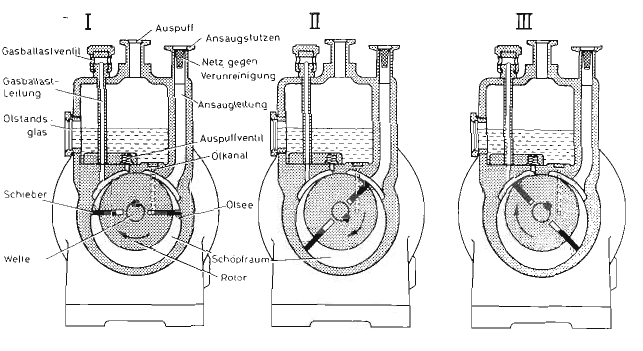
\includegraphics[scale=0.7]{./fig/massenspek_drehschieber.png}
 \caption{Skizze einer Drehschieberpumpe (Quelle: \cite[S. 7]{Litmap})}
 \label{fig011}
\end{figure}

\subsection{Turbomolekularpumpe}

Eine Turbomolekularpumpe besteht aus einer Statoreinheit und einer Rotoreinheit. Die Rotoreinheit besteht aus einzelnen Schaufeln, die unter einem Winkel $\alpha$ gegen die Diffusionsrichtung gestellt sind.
Die Schaufeln rotieren mit einer Geschwindigkeit $u$, die (am äußeren Rand) ungefähr der mittleren thermischen Geschwindigkeit der Gasmoleküle entspricht. Durch die wiederholte Kollision der Gasmoleküle mit den Rotorschaufeln erhalten diese einen Impuls in Pumprichtung.
Oft sind Turbomolekularpumpen auch aus mehreren hintereinander geschalteten Pumpstufen aufgebaut.

\section{Quadrupol-Massenspektrometer}

In diesem Versuch wird ein Quadrupol-Massenspektrometer (s. Abb. \ref{fig021}) verwendet. Es besteht aus vier hyperbelförmigen Elektroden. Diese erzeugen eine Überlagerung aus einem Gleichfeld $\phi_{1}=U$ und einem Wechselfeld $\phi_{2}=V\cos(\omega t)$.
Die Ionen werden so zwischen den Elektroden auf eine Wellenbahn gezwungen. Das Verhältnis $\frac{U}{V}$ lässt sich so einstellen, dass nur Ionen, die ein bestimmtes Verhältnis $\frac{m}{q}$ der Masse $m$ zur Ladung $q$ besitzen, die Elektroden passieren. Ionen einer anderen Masse stoßen an die Elektroden, und können den Filter nicht passieren.

\begin{figure}[tb]
 \centering
 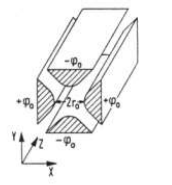
\includegraphics[scale=0.9]{./fig/massenspek_quadrupol.png}
 \caption{Schematische Skizze eines Quadrupol-Massenfilters (Quelle: \cite[S. 25]{Litmap})}
 \label{fig021}
\end{figure}

\section{Ionisationsvakuummeter}

Ein Ionisationsvakuummeter ist ein Messgerät, dass zur Messung niedriger Drücke (im Bereich $1$ bis $\SI{e-11}{\milli\bar}$) eingesetzt wird. Zur Messung des Druckes wird mittels einer Glühkathode ein Elektronenstrom erzeugt. Dieser wird über eine Strecke $\Delta l$ durch das Gas zu einem Ionenfänger geleitet.
Die Elektronen stoßen dabei mit den Gasteilchen zusammen und ionisieren diese. Für den dadurch auftretenden Ionenstrom $I^{+}$ gilt
\begin{equation}
 I^{+} = I^{-}S\Delta l,
\end{equation}
mit dem Elektronenstrom $I^{-}$ und der differentiellen Ionisierung $S=n\sigma$, wobei $n$ die Teilchenzahldichte der Gasteilchen und $\sigma$ den Wirkungsquerschnitt des Stoßes bezeichnen.
Für den Zusammenhang von $I^{+}$ mit dem Gasdruck $p$ ergibt sich
\begin{equation}
 I^{+} = \varepsilon I^{-}p,
\end{equation}
mit der Vakuummeterkonstante $\varepsilon$, die von der Geometrie des Messgeräts abhängt.

\section{Ionenquellen}

Zur Untersuchung der Moleküle ist es notwendig, diese zu ionisieren. Dies kann mit Hilfe folgender Methoden erreicht werden.
\begin{itemize}
 \item Stoßionisation: Diese Methode wird im Versuch verwendet. Hierbei werden die Gasmoleküle mit Elektronen beschossen. Beim Stoß der Elektronen mit den Gasmolekülen kann es zur Ionisation kommen.
 Außerdem kann es zur Dissoziation eines Moleküls kommen. Dies ist wahrscheinlicher, falls sich das Molekül in einem hochangeregten Schwingungszustand befindet.
 \item Thermische Oberflächenionisation: Von einer heißen Metalloberfläche dampfen adsorbierte Moleküle mit hoher Wahrscheinlichkeit als Ionen ab.
 \item Feldionisation: Hierbei werden die Moleküle in ein stark inhomogenes elektrisches Feld gebracht. Durch den quantenmechanischen Tunneleffekt kann es dabei zur Ionisation kommen.
\end{itemize}


\section{Versuch 1: Einführung}

In diesem Versuch wird zunächst ein Restgasspektrum unter Standardbedingungen ($E=\SI{65}{\electronvolt}, \, I^{-}=\SI{1}{\milli\ampere}$) aufgenommen. Der Versuchsaufbau ist in Abb. \ref{fig0v11} dargestellt.
Es werden Linien bei $m=28,\, 32$ und $44$ erwartet. Diese gehören vermutlich zu $\textrm{N}_{2}, \, \textrm{O}_{2}$ und $\textrm{CO}_{2}$.

Für eine Linie wird die Abhängigkeit des Ionenstroms $I^{+}$ vom Elektronenstrom $I^{-}$ gemessen. Es wird erwartet, dass der Ionenstrom mit steigendem Elektronenstrom ansteigt.

\begin{figure}[tb]
 \centering
 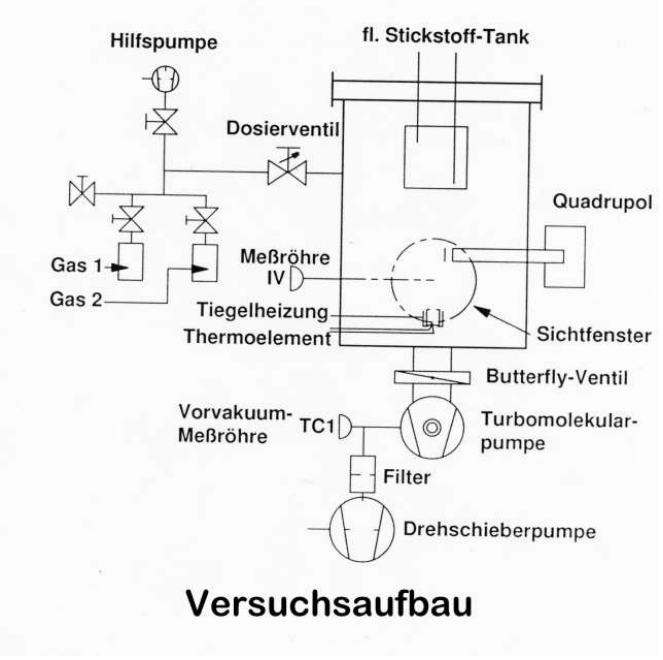
\includegraphics[scale=0.5]{./fig/massenspek_aufbau.png}
 \caption{Schematische Skizze des Versuchsaufbaus (Quelle: \cite[S. 4]{Litmap})}
 \label{fig0v11}
\end{figure}

\subsection{Auflösungsvermögen}

Des Weiteren wird in diesem Versuch das Auflösungsvermögen $R=\frac{m}{\Delta m}$ an jeweils einer Linie im Bereich großer und kleiner Massenzahlen gemessen. Es gibt dabei drei verschiedene Methoden, das Auflösungsvermögen zu definieren.
\begin{enumerate}
 \item Die \%-Anteil Definition: Zwei Linien werden als getrennt bezeichnet, wenn der gegenseitige Anteil der Höhe $x\%$ der Maximalhöhe nicht überschreitet.
 \item Die \%-Tal Definition: Zwei gleichhohe Linien werden als getrennt bezeichnet, wenn die Höhe des Tals zwischen ihnen $x\%$ nicht überschreitet.
 \item Die \%-Linienbreite Definition: Hier ergibt sich $\Delta m$ durch die Linienbreite in $x\%$ Höhe.
\end{enumerate}
In diesem Versuch wird die \%-Linienbreite Definition verwendet werden, da diese auch für alleinstehende Linien anwendbar ist. Es wird erwartet, dass das Auflösungsvermögen in Abhängigkeit von $m$ steigt, da die Linienbreite in Abhängigkeit von $m$ konstant bleiben sollte.

\section{Versuch 2: Auftrittsenergie von Argon}

In diesem Versuch werden die Auftrittsenergien von Ar$^{+}$ und Ar$^{2+}$ gemessen. Bei der Auftrittsenergie handelt es sich um die Energie der stoßenden Elektronen, ab der die Ionisierung stattfindet.
Dazu wird Argon mit dem Dosierventil bei angeschlossener Turbomolekularpumpe bis zu einem Maximaldruck von $\SI{5e-6}{\milli\bar}$ in den Rezipienten geleitet. Es werden Linien bei $m=40$ (Ar$^{+}$) und $m=20$ (Ar$^{2+}$) erwartet. Dies liegt daran, dass nicht direkt die Massen, sondern das Verhältnis $\frac{q}{m}$ gemessen wird, was bei Ar$^{2+}$ Ionen zu einer scheinbar halb so großen Masse führt.

\section{Versuch 3: Dissoziationsenergien von Stickstoff}
\label{sec:v3}

In diesem Versuch werden die Dissoziationsenergien für das neutrale Stickstoffmolekül und für das Stickstoffmolekülion bestimmt. Unter Elektronenbeschuss sind die folgenden Reaktionswege möglich
\begin{align}
 \textrm{N}_{2} \, + \, \textrm{e}^{-} \, &\to \, \textrm{N}_{2}^{+} \, + \, 2\textrm{e}^{-}, \\
 \textrm{N}_{2} \, + \, \textrm{e}^{-} \, &\to \, \textrm{N}^{+} \, + \, \textrm{N} \, + \, 2\textrm{e}^{-}, \\
 \textrm{N}_{2}^{+} \, + \, \textrm{e}^{-} &\, \to \, 2\textrm{N}^{+} \, + \, 2\textrm{e}^{-}.
\end{align}
Durch Messung der Auftrittsenergien für $m=14$ und $m=28$ können nun die Dissoziationsenergien bestimmt werden. Für diese ergibt sich
\begin{align*}
 E_{\textrm{D}}(\textrm{N}_{2}) &= E_{\textrm{A}}(\textrm{N}^{+}) - E_{\textrm{I}}, \\
 E_{\textrm{D}}(\textrm{N}_{2}^{+}) &= E_{\textrm{A}}(\textrm{N}^{+}) - E_{\textrm{A}}(\textrm{N}_{2}^{+}),
\end{align*}
wobei $E_{\textrm{D}}$ die Dissoziationsenergie, $E_{\textrm{A}}$ die Auftrittsenergie und $E_{\textrm{I}}$ die Ionisationsenergie bezeichnet.




\section{Versuch 4: Quantitative Analyse}

Da sich Moleküle unterschiedliche Ionisierungsenergien habe und sich somit die verschiedenen Ionenströme nicht gegenseitig beeinflussen, lässt sich eine 
quantitative Analyse eines Gasgemischs durchführen. Die Massenspektren überlagern
sich additiv, wodurch von der Höhe des Ionenstroms auf den relativen Anteil der einzelnen Moleküle geschlossen werden kann.\\
Als erstes wird für eventuell nötige Korrekturen ein Untergrundspektrum für m = 14 u und m = 28 u aufgenommen.
Danach wird Raumluft bis $5\cdot10^{-6} \si{\bar}$ in die Kammer eingelassen und erneut ein Massenspektrum aufgenommen, woraus die Partialdrücke der einzelnen Moleküle bestimmt werden können.\\
Summiert man die Partialdrücke auf wird der Gesamtdruck vermutlich niedriger als der gemessene Druck in der Ionisationskammer sein, da nur ein Bruchteil der Moleküle tatsächlich ionisiert wird und am Detektor erfasst werden kann.

\section{Versuch 5: Qualitative Analyse}

Für die qualitative Analyse wird ein unbekanntes Kohlenwasserstoffmolekül in die Ionisationskammer eingelassen und bei E = {15, 30, 65}\;eV jeweils ein Massenspektrum aufgenommen.
Das große Molekül dissoziiert dabei in kleinere ionisierte Bruchstücke, die bestimmt werden sollen.\\
Es wird erwartet, dass die Anzahl der Bruchstücke mit steigender Energie zunimmt, da bei höheren kinetischen Energien der stoßenden Elektronen mehr Energie auf die Molekülbindungen übertragen wird. 
Übersteigt diese Energie die benötigte Dissoziationsenergie dieser Bindung zerbricht das Molekül in kleinere ionisierte Bruchstücke.

\section{Versuch 6: Restgasanalyse}

In diesem Versuch wird erneut eine Massenspektrum aufgenommen und daraus quantitativ die Bestandteile des Restgases in der Ionisationskammer bestimmt.
Nachdem die Kammer auf 77\;K herunter gekühlt wurde, wird erwartet, dass die Summe der Partialdrücke geringer als bei Raumtemperatur ist, da zB Wasserdampf bei solch niedrigen Temperaturen fest wird und somit nicht mehr als einzelne Ionen am Detektor gemessen werden kann.

\xtable{htb}{tab_vorlage_multicolumn}{Totzeit der Versuche}{}